\subsection{Выбор инструментов разработки}\label{subsec:development_tools}
Рекомендательные алгоритмы реализовывались на языке Python~\cite{python}.
Выбор обусловлен наличием большого количества библиотек для работы с математическими вычислениями, алгоритмами машинного обучения и нейросетями, а также лёгкость прототипирования на нём.
Основные используемые библиотеки:
\begin{itemize}
    \item \textbf{NumPy}~\cite{numpy} --- для работы с матричными вычислениями;
    \item \textbf{pandas}~\cite{pandas} --- для работы с большими объёмами данных, в том числе для предобработки;
    \item \textbf{scikit-learn}~\cite{scikit-learn} --- для организации обучения моделей машинного обучения: разбиение данных на обучающую и тестовую выборки, вычисление метрик;
    \item \textbf{Matplotlib}~\cite{matplotlib} --- для построения графиков;
    \item \textbf{TensorFlow}~\cite{tensorflow} --- для обучения нейросетевых моделей.
\end{itemize}

Python --- интерпретируемый язык.
Эта категория языков, как правило, медленнее компилируемых.
Однако, библиотеки, реализующие сложные математические вычисления, написаны на компилируемых языках, таких как С~\cite{c-language} или C++~\cite{c++}.
Это делает код, использующий эти библиотеки, очень быстрым.
Таким образом, в данном контексте выбор Python в качестве языка программирования упрощает разработку, сохраняя при этом производительность программ.

\pagebreak
\subsection{Структура проекта}\label{subsec:project_structure}
Каждый рекомендательный алгоритм представляет из себя отдельную модель (класс).
Все модели наследуются от базового класса, в котором реализована общая функциональность, сопутствующая обучению:
\begin{itemize}
    \item Предобработка данных;
    \item Инициализация модели;
    \item Разбиение данных на обучающую и тестовую выборки;
    \item Построение графиков и мониторинг процесса обучения;
    \item Сохранение параметров обучения модели и её выхода;
    \item Оценка качества модели;
    \item Поиск гиперпараметров (таких как размерность векторных представлений или количество эпох обучения), дающих наилучшее качество.
\end{itemize}

Каждый класс содержит в себе программную реализацию конкретного алгоритма.
В отдельных пакетах реализуются загрузка данных и метрики оценивания.

Самым важным на этапе исследования является подбор гиперпараметров модели, приводящих к оптимальному качеству.
Поиск оптимальных гиперпараметров представлен на блок-схеме~\ref{fig:params_search_diagram}:

\begin{figure}[h!]
\centering
\begin{minipage}{0.9\textwidth}
\centering
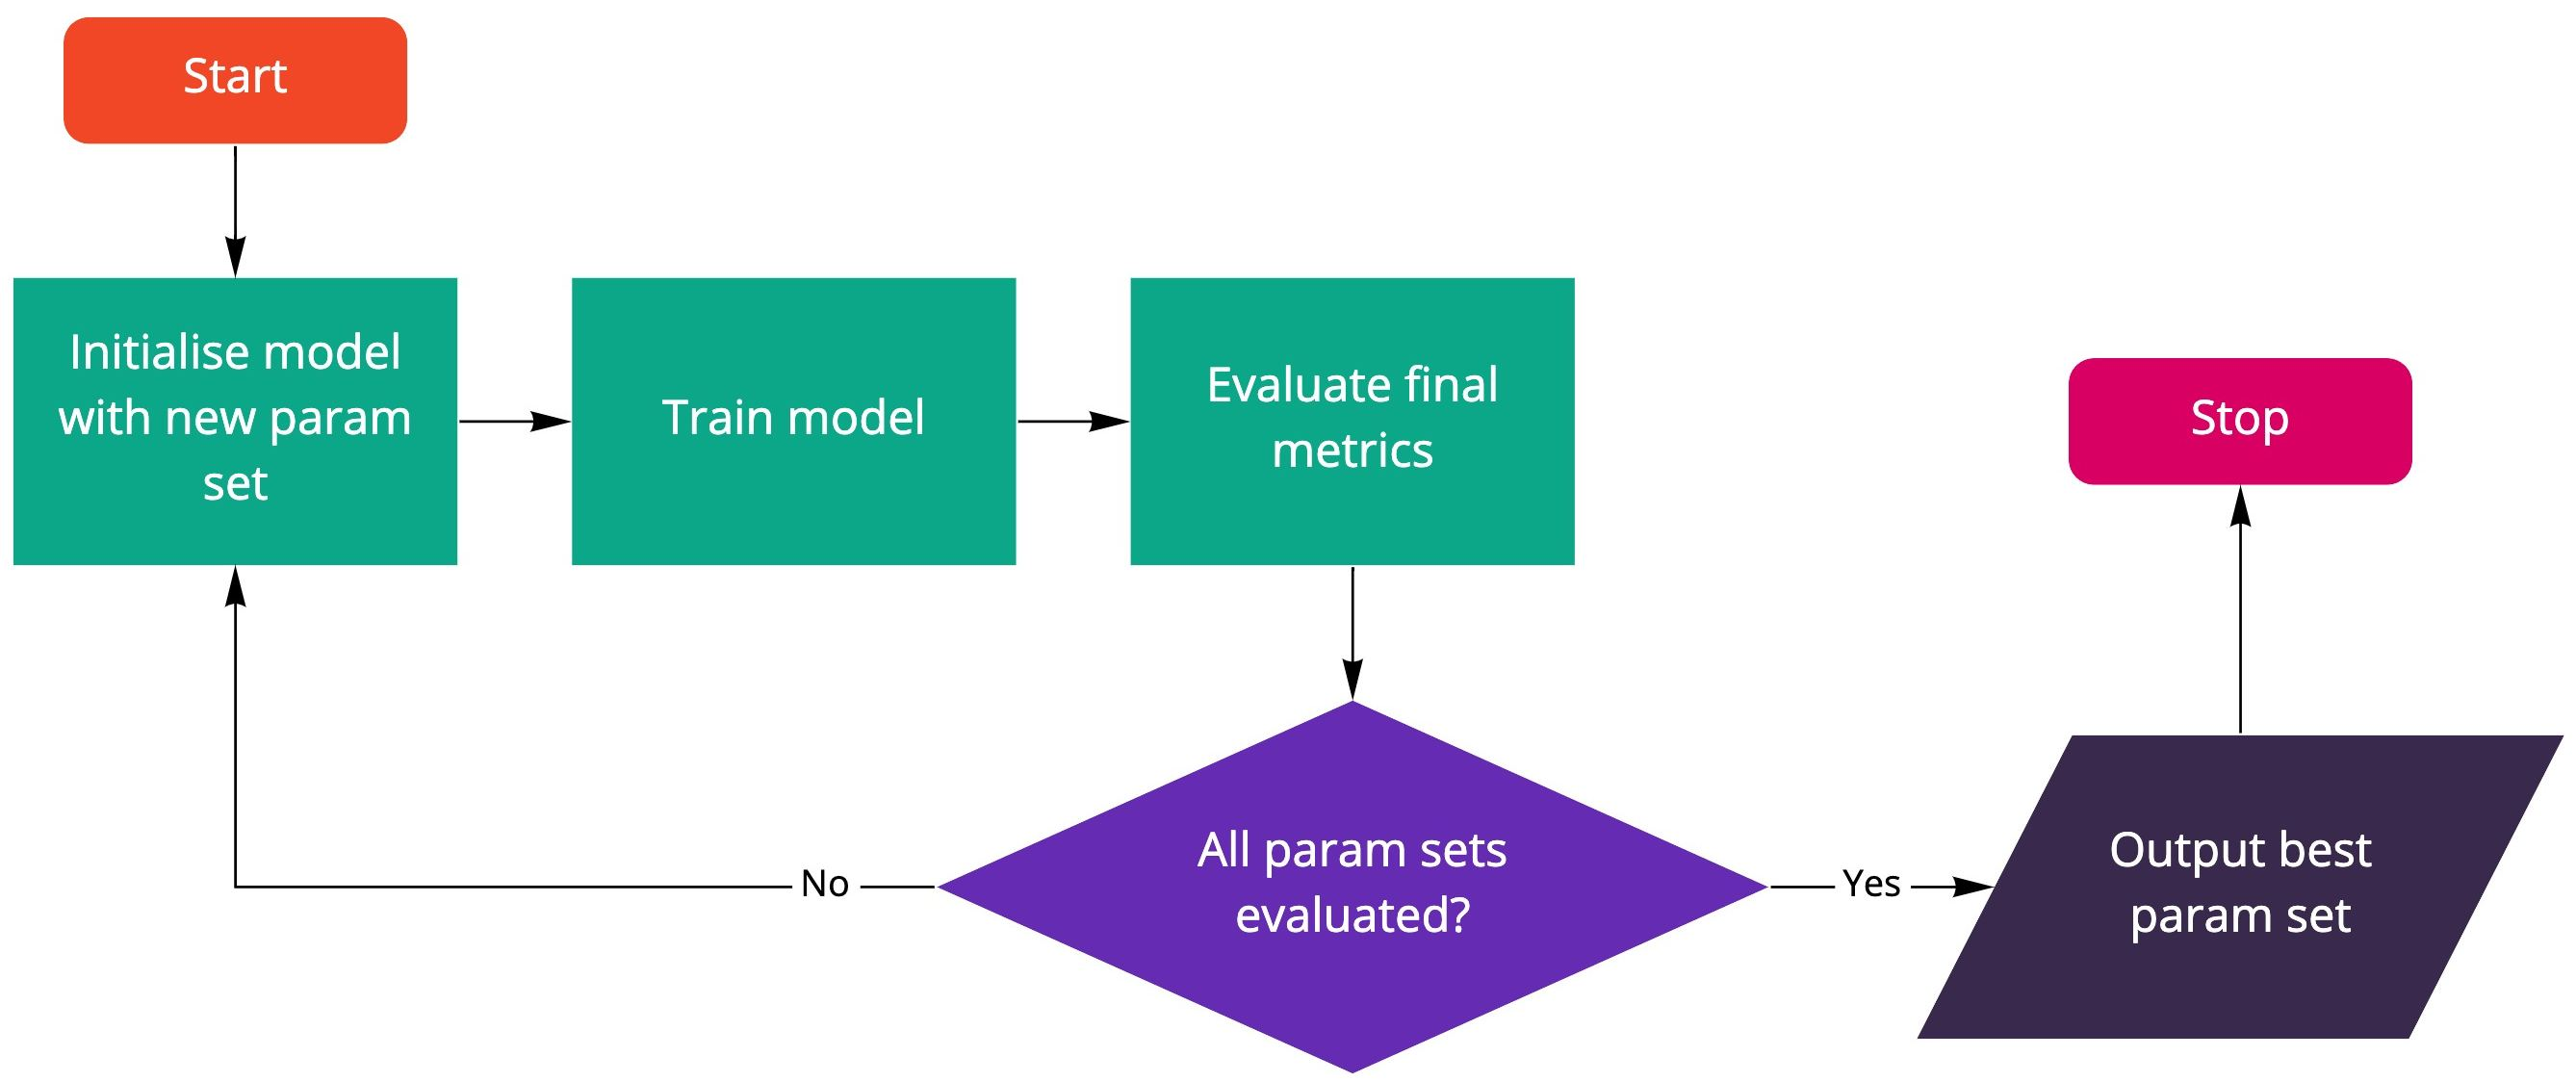
\includegraphics[width=0.9\linewidth]{images/params_search_diagram}
\caption{Поиск оптимальных гиперпараметров}
\label{fig:params_search_diagram}
\end{minipage}
\end{figure}

\pagebreak
Процесс обучения модели с конкретным набором гиперпараметров в общем виде представлен на блок-схеме~\ref{fig:train_model_diagram}:

\vspace{1em}
\begin{figure}[h!]
\centering
\begin{minipage}{0.9\textwidth}
\centering
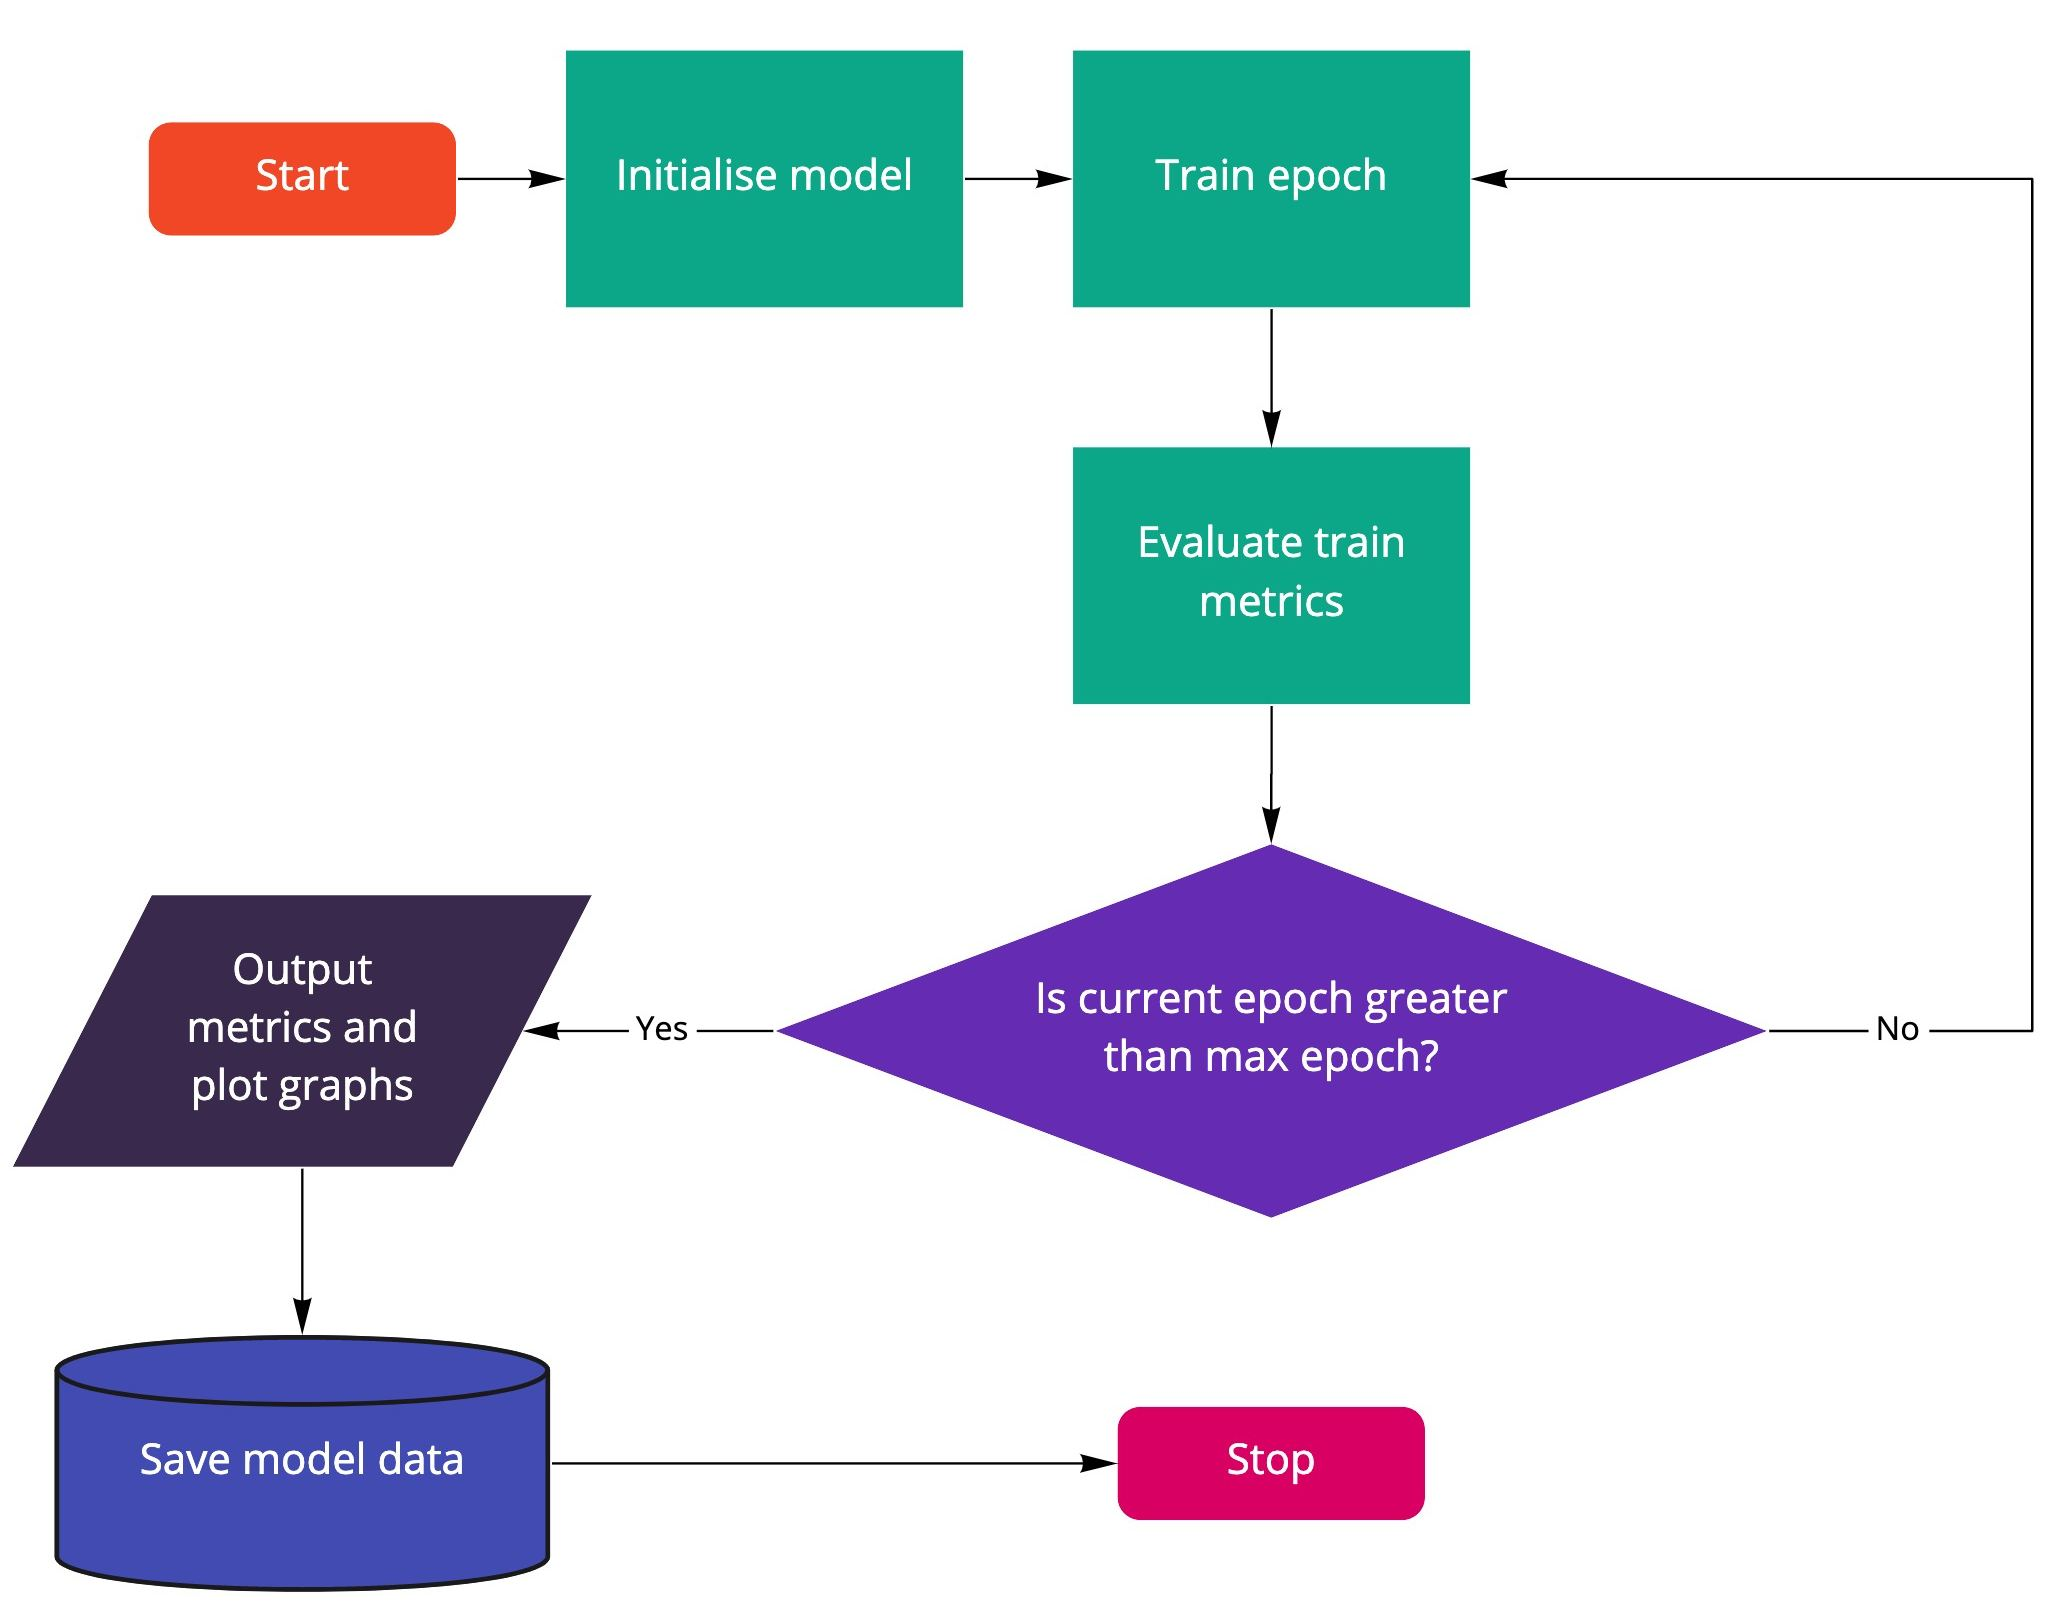
\includegraphics[width=0.9\linewidth]{images/train_model_diagram}
\caption{Процесс обучения модели}
\label{fig:train_model_diagram}
\end{minipage}
\end{figure}

Код проекта доступен по ссылке: \url{https://github.com/shumoff/diploma}.

\pagebreak
\subsection{Архитектура моделей}\label{subsec:models_architecture}
Для поиска набора гиперпараметров, дающего оптимальное качество алгоритма, использовались данные из MovieLens 20M Dataset~\cite{movielens-dataset}.
Датасет содержит 20 миллионов оценок и 465 тысяч тегов, поставленных 138 тысячами пользователей 27 тысячам фильмов.
Обучение производилось на 1 миллионе оценок, поставленных 6 тысячами пользователей 5 тысячам фильмов.
Примеры исходных данных приведены в таблицах~\ref{table:ratings_data},~\ref{table:tags_data}:

\begin{table}[h]
    \begin{minipage}{.5\linewidth}
      \centering
        \begin{tabular}{|P{1.5cm}|P{2cm}|P{2cm}|}
            \hline
            userId & movieId & rating\\
            \hline
            438 & 5055 & 4.0\\
            \hline
            462 & 8910 & 3.0\\
            \hline
            474 & 3793 & 4.5\\
            \hline
            559 & 518 & 2.0\\
            \hline
        \end{tabular}
        \caption{Данные по оценкам}
        \label{table:ratings_data}
    \end{minipage}%
    \begin{minipage}{.5\linewidth}
      \centering
        \begin{tabular}{|P{1.5cm}|P{2cm}|P{3cm}|}
        \hline
            userId & movieId & tag\\
            \hline
            62 & 7153 & fantasy\\
            \hline
            318 & 778 & dark comedy\\
            \hline
            424 & 1625 & plot twist\\
            \hline
            474 & 140 & journalism\\
           \hline
        \end{tabular}
        \caption{Данные по тегам}
        \label{table:tags_data}
    \end{minipage}
\end{table}

%\subsubsection{ALS}
\paragraph{ALS}
Набор гиперпараметров модели:
\begin{itemize}
    \item $N$ --- количество эпох обучения;
    \item $D$ --- размерность пространства векторных представлений;
    \item $\lambda_{U}$, $\lambda_{V}$ --- параметры регуляризации.
\end{itemize}

Гиперпараметры модели, дающие наилучшее качество, приведены в таблице~\ref{tab:als_params}:
\begin{table}[h]
    \centering{
    \begin{tabular}{ |P{4.5em}|P{4.5em}|P{4.5em}|P{4.5em}|P{4.5em}|P{4.5em}|}
    \hline
    $N$ & $D$ & $\lambda_{U}$ & $\lambda_{V}$ \\
    \hline
    40 & 100 & 6 & 6.5 \\
    \hline
    \end{tabular}}
    \caption{Гиперпараметры ALS}
    \label{tab:als_params}
\end{table}

\pagebreak
%\subsubsection{SGD}
\paragraph{SGD}
Набор гиперпараметров модели:
\begin{itemize}
    \item $N$ --- количество эпох обучения;
    \item $D$ --- размерность пространства векторных представлений;
    \item $\nu$ --- коэффициент скорости обучения;
    \item $\lambda_{U}$, $\lambda_{V}$ --- параметры регуляризации.
\end{itemize}

Гиперпараметры модели, дающие наилучшее качество, приведены в таблице~\ref{tab:sgd_params}:
\begin{table}[h]
    \centering{
    \begin{tabular}{ |P{4.5em}|P{4.5em}|P{4.5em}|P{4.5em}|P{4.5em}|P{4.5em}|}
    \hline
    $N$ & $D$ & $\nu$ & $\lambda_{U}$ & $\lambda_{V}$ \\
    \hline
    70 & 80 & 0.01 & 0.1 & 0.01 \\
    \hline
    \end{tabular}}
    \caption{Гиперпараметры SGD}
    \label{tab:sgd_params}
\end{table}


%\subsubsection{PMF}
\paragraph{PMF}
Набор гиперпараметров модели:
\begin{itemize}
    \item $N$ --- количество эпох обучения;
    \item $D$ --- размерность пространства векторных представлений;
    \item $\nu$ --- коэффициент скорости обучения;
    \item $\sigma_{U}$, $\sigma_{V}$ --- дисперсия для первоначальной инициализации векторов пользователей и объектов.
\end{itemize}

Гиперпараметры модели, дающие наилучшее качество, приведены в таблице~\ref{tab:pmf_params}:
\begin{table}[h]
    \centering{
    \begin{tabular}{ |P{4.5em}|P{4.5em}|P{4.5em}|P{4.5em}|P{4.5em}|P{4.5em}|}
    \hline
    $N$ & $D$ & $\nu$ & $\sigma_{U}$ & $\sigma_{V}$ \\
    \hline
    50 & 20 & 0.001 & 0.3 & 0.3 \\
    \hline
    \end{tabular}}
    \caption{Гиперпараметры PMF}
    \label{tab:pmf_params}
\end{table}

%\subsubsection{Нейронная сеть}
\paragraph{Нейронная сеть}
Архитектура нейросети представлена на рисунке~\ref{fig:nn_arch}:
\begin{figure}[h!]
\center{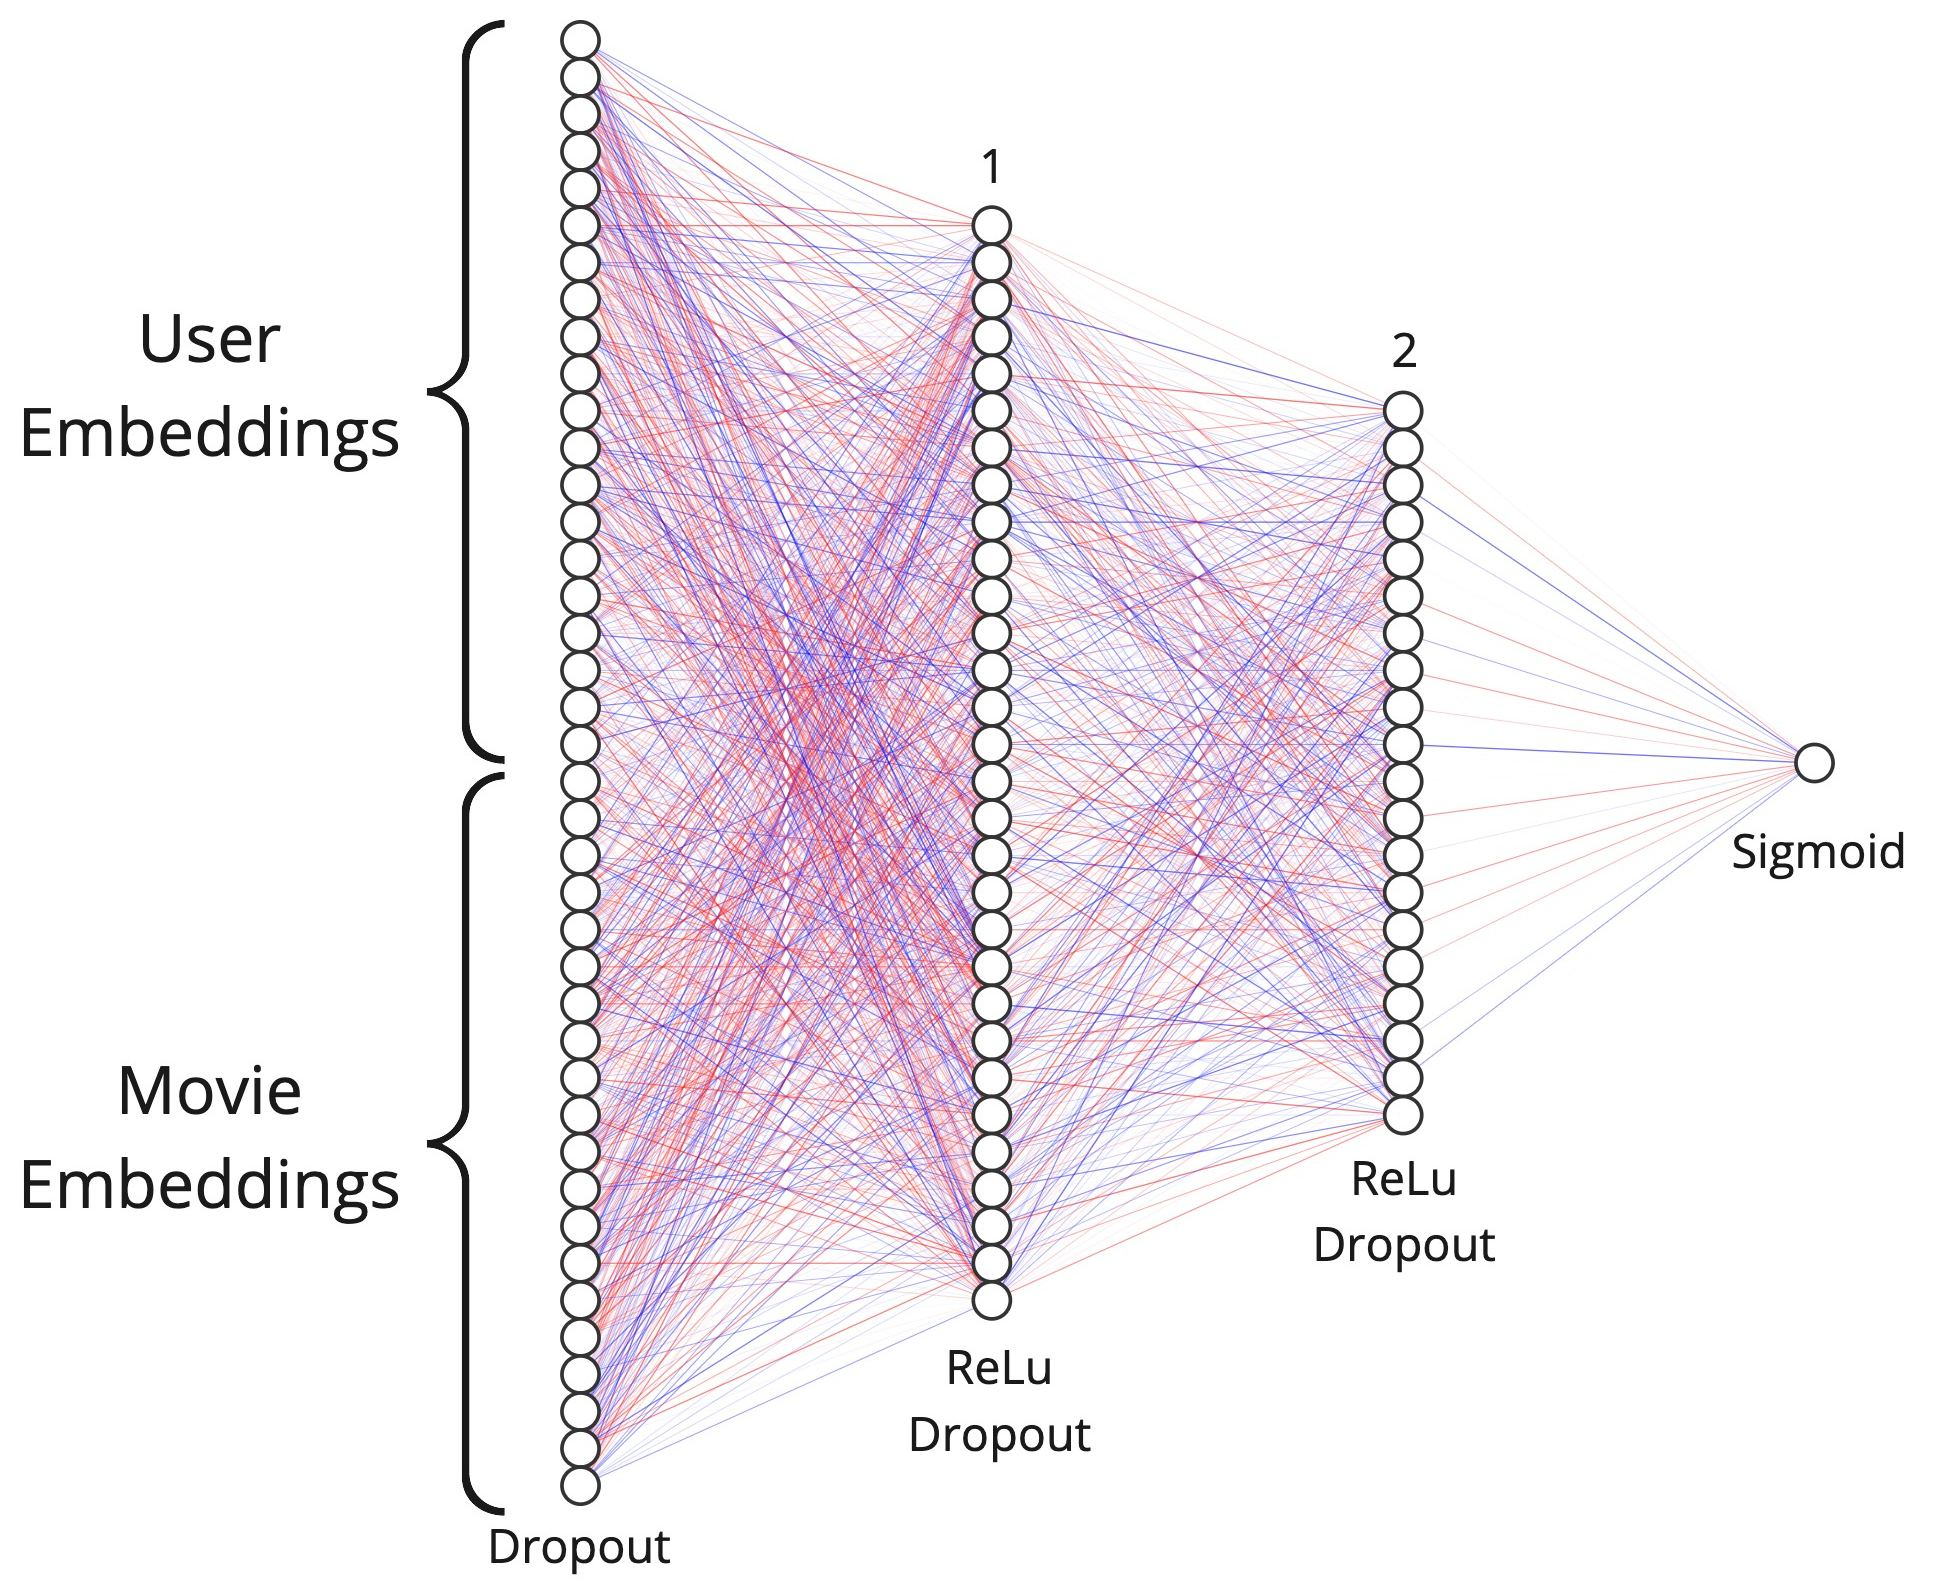
\includegraphics[scale=0.2]{images/nn_arch}}
\caption{}
\label{fig:nn_arch}
\end{figure}

Для защиты от переобучения используется техника исключения определённого процента случайных нейронов --- Dropout~\cite{dropout}.

В качестве функции активации нейрона используются линейный выпрямитель (ReLU)~\cite{relu}:
\begin{equation}
f(x) =
\begin{cases}
    0, & x < 0 \\
    x, & x \geq 0
\end{cases}\label{eq:relu}
\end{equation}

А также логистическая функция:
\begin{equation}
    f(x) = \frac{1}{1 + e^{-x}}\label{eq:sigmoid}
\end{equation}

\pagebreak
Графики функций активации представлены на рисунках~\ref{fig:relu},~\ref{fig:sigmoid}:
\begin{figure}[h!]
\centering
\begin{minipage}{.5\textwidth}
\centering
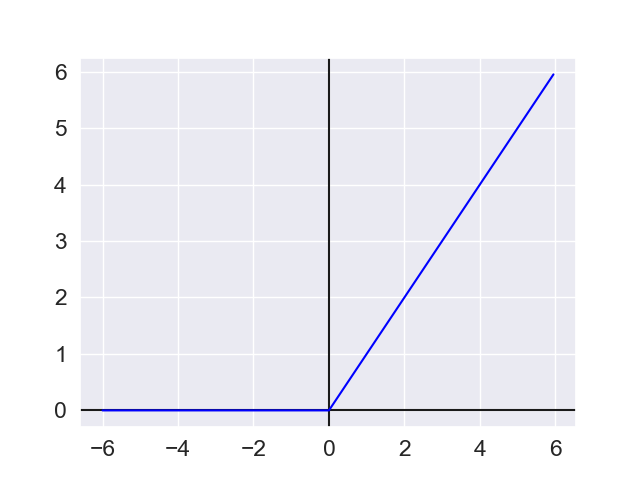
\includegraphics[width=1.0\linewidth]{images/relu}
\caption{Rectified linear unit}
\label{fig:relu}
\end{minipage}%
\begin{minipage}{.5\textwidth}
\centering
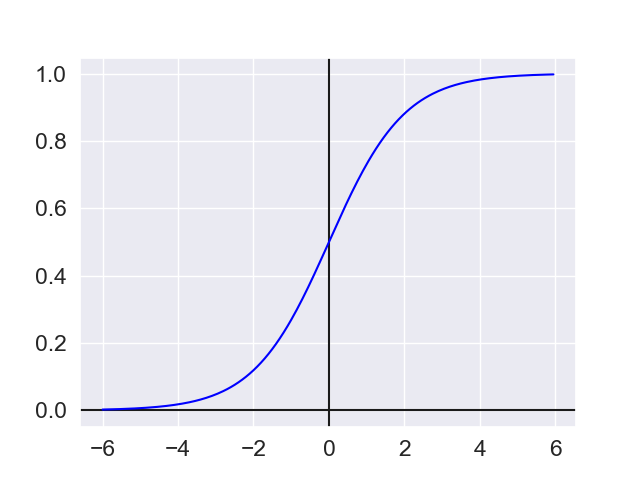
\includegraphics[width=1.0\linewidth]{images/sigmoid}
\caption{Логистическая функция}
\label{fig:sigmoid}
\end{minipage}
\end{figure}

Набор гиперпараметров, по которым производился поиск:
\begin{itemize}
    \item $N$ --- количество эпох обучения;
    \item $D$ --- размерность пространства векторных представлений;
    \item $\nu$ --- коэффициент скорости обучения;
    \item $k_1$, $k_2$ --- количество нейронов в скрытых слоях 1 и 2.
\end{itemize}

Гиперпараметры модели, дающие наилучшее качество, приведены в таблице~\ref{tab:nn_params}:
\begin{table}[h]
    \centering{
    \begin{tabular}{ |P{4.5em}|P{4.5em}|P{4.5em}|P{4.5em}|P{4.5em}|P{4.5em}|}
    \hline
    $N$ & $D$ & $\nu$ & $k_1$ & $k_2$ \\
    \hline
    15 & 100 & 0.002 & 150 & 100 \\
    \hline
    \end{tabular}}
    \caption{Гиперпараметры нейросети}
    \label{tab:nn_params}
\end{table}

\pagebreak
%\subsubsection{Контентная модель}
\paragraph{Контентная модель}
Для выделения контентных признаков объектов использовались тэги, присвоенные пользователями фильмам.
Сначала для корпуса тэгов было построено TF-IDF пространство, а затем сжато путём кодирования автоэнкодером.
В качестве функции активации нейрона используются ReLU и логистическая функция.
Для защиты от переобучения используется Dropout.

Архитектура автоэнкодера представлена на рисунке~\ref{fig:autoencoder}:
\begin{figure}[h!]
    \center{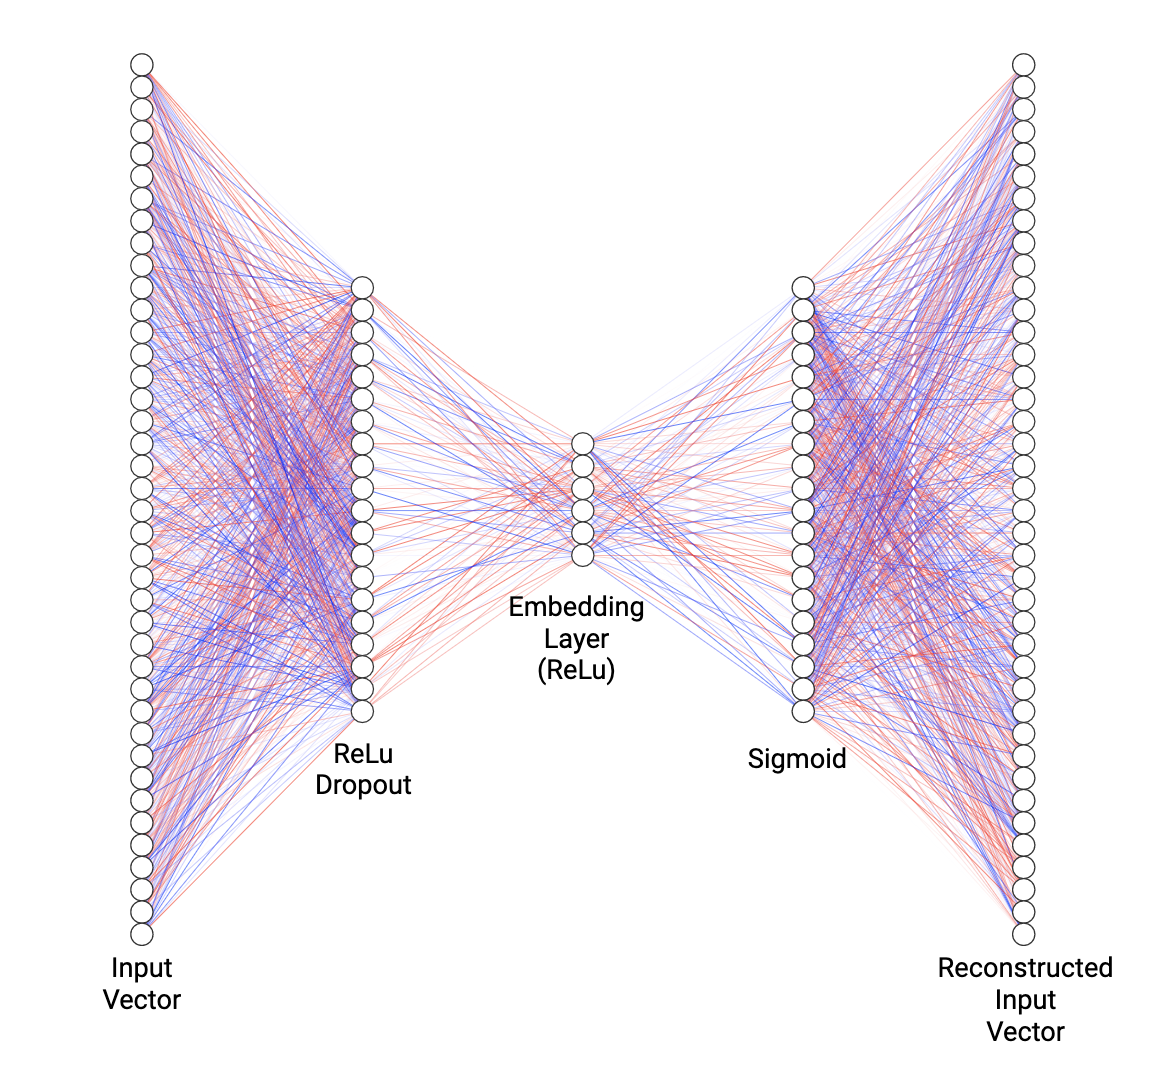
\includegraphics[scale=0.75]{images/autoencoder}}
    \caption{}
    \label{fig:autoencoder}
\end{figure}

\pagebreak
Набор гиперпараметров, по которым производился поиск:
\begin{itemize}
    \item $N$ --- количество эпох обучения;
    \item $D$ --- размерность пространства векторных представлений;
    \item $\nu$ --- коэффициент скорости обучения;
    \item $k$ --- количество нейронов в скрытом слое.
\end{itemize}

Гиперпараметры модели, дающие наилучшее качество, приведены в таблице~\ref{tab:autoencoder_params}:
\begin{table}[h]
    \centering{
    \begin{tabular}{ |P{4.5em}|P{4.5em}|P{4.5em}|P{4.5em}|P{4.5em}|P{4.5em}|}
    \hline
    $N$ & $D$ & $\nu$ & $k$ \\
    \hline
    20 & 100 & 0.001 & 5000 \\
    \hline
    \end{tabular}}
    \caption{Гиперпараметры автоэнкодера}
    \label{tab:autoencoder_params}
\end{table}

\pagebreak
\subsection{Работа рекомендательной системы}\label{subsec:recommendations_obtaining}
Гибридная рекомендательная система сочетает в себе две модели: коллаборативную и контентную.
Это позволяет предлагать пользователю релевантные объекты, отбирать объекты, похожие на объект интереса, и задавать порядок ранжирования, используя знания обоих моделей.
Процесс работы такой системы представлен на блок-схеме~\ref{fig:hybrid_system_diagram}:

\vspace{1em}
\begin{figure}[h!]
\centering
\begin{minipage}{0.9\textwidth}
\centering
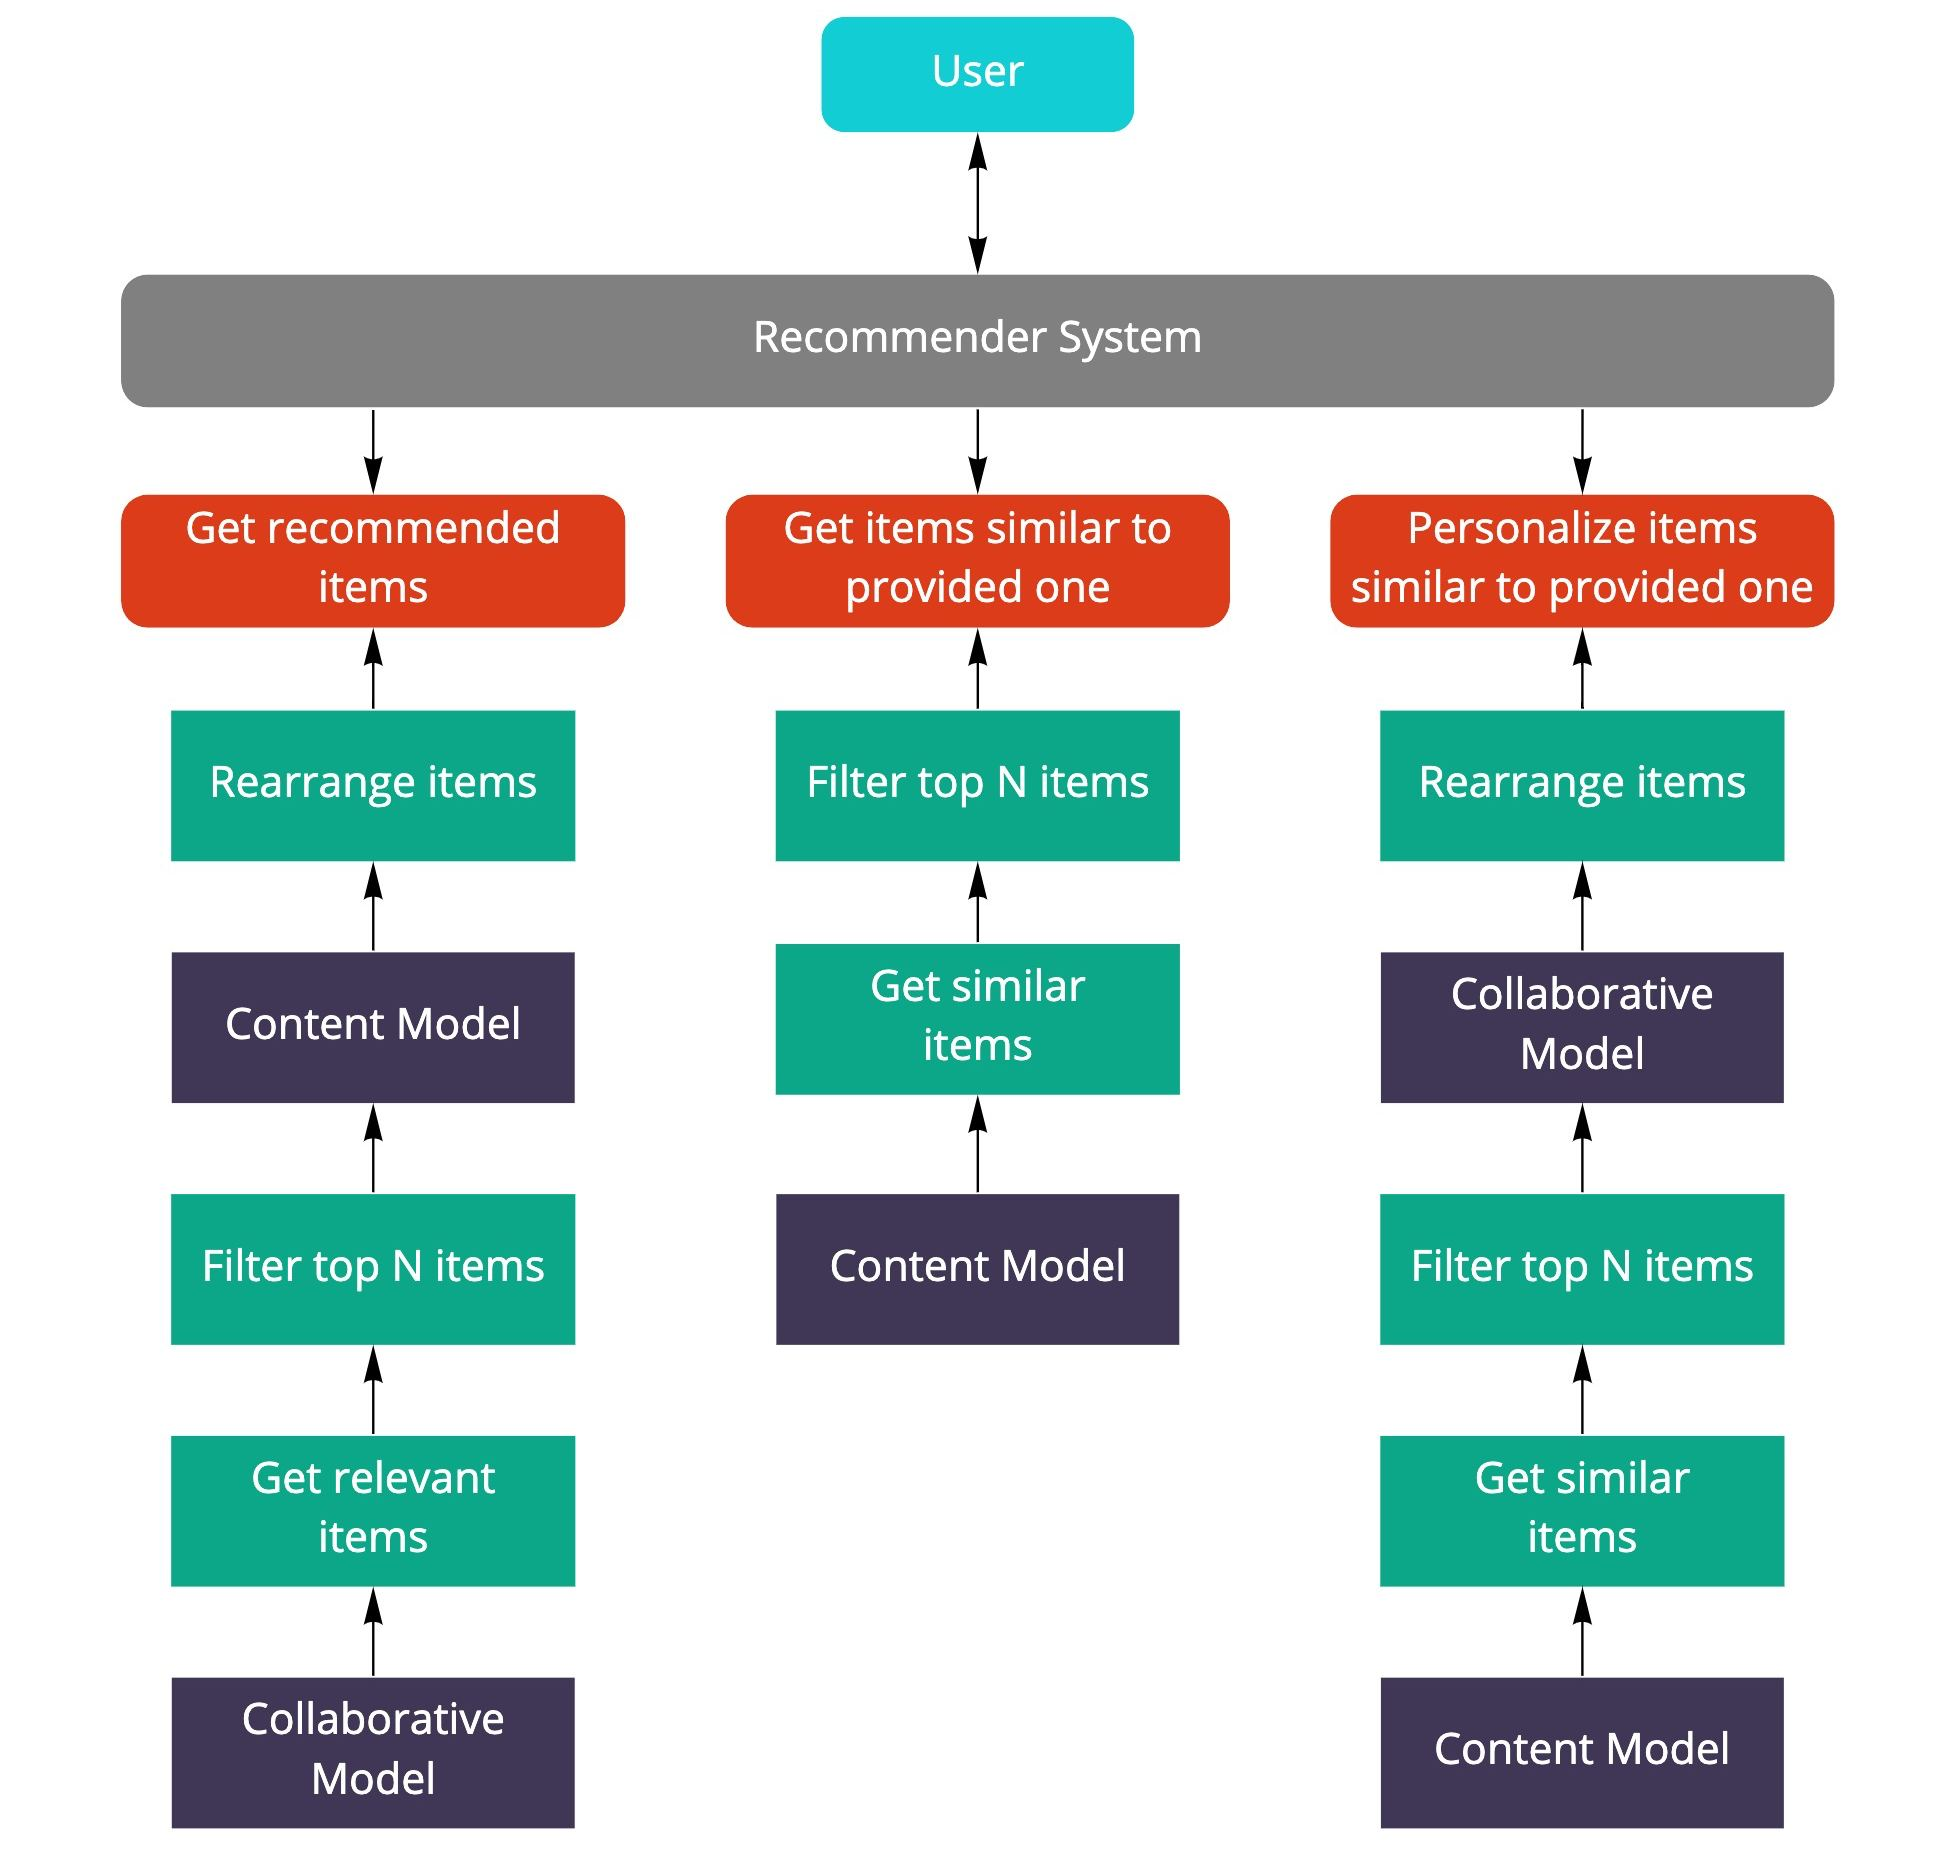
\includegraphics[width=0.9\linewidth]{images/hybrid_system_diagram}
\caption{Схема гибридной рекомендательной системы}
\label{fig:hybrid_system_diagram}
\end{minipage}
\end{figure}
